\documentclass[conference]{IEEEtran}

\usepackage{cite}
\usepackage{amsmath,amssymb,amsfonts}
\usepackage{graphicx}
\usepackage{textcomp}
\usepackage{xcolor}
\usepackage{booktabs}
\usepackage{listings}
\usepackage{hyperref}
\usepackage{balance}

\lstset{
  language=Python,
  basicstyle=\ttfamily\scriptsize,
  keywordstyle=\color{blue},
  commentstyle=\color{gray},
  stringstyle=\color{red!60!black},
  showstringspaces=false,
  frame=single,
  breaklines=true,
  numbers=none,
  xleftmargin=2mm,
  xrightmargin=2mm,
}

\begin{document}

\title{3we: An Open Infrastructure for Sim-to-Real Embodied AI Research}

\author{\IEEEauthorblockN{3we Contributors}
\IEEEauthorblockA{Open Source Project\\
\url{https://github.com/3we-org/3we-robot-platform}}}

\maketitle

% ===========================================================================
\begin{abstract}
Embodied AI research requires tight integration of simulation, real hardware, and learning algorithms---yet existing platforms force researchers to choose between expensive proprietary systems, simulation-only environments, or hardware platforms with steep ROS2 learning curves.
We present \textbf{3we}, a fully open-source infrastructure where the same Python code runs identically across a lightweight mock simulator, Gazebo, NVIDIA Isaac Sim, and real hardware (Raspberry Pi~5 + Hailo-8L) with zero modification.
The platform provides an AI-First Python API that reduces typical ROS2 navigation code from 60+ lines to 5, Gymnasium-compatible environments, native VLM/VLA integration, and standardized benchmarks across 7 evaluation scenes.
On reproducible hardware costing under \$300 (BOM), we demonstrate Sim-to-Real transfer ratios exceeding 0.6 on point navigation tasks and provide community baselines achieving 82\% success rate (SPL 0.65) in structured environments.
All software (Apache~2.0), hardware designs (CERN-OHL-P~v2), and documentation (CC-BY-SA~4.0) are publicly available.
\end{abstract}

% ===========================================================================
\section{Introduction}

Embodied AI---the study of intelligent agents that perceive and act in physical environments---has emerged as a central challenge in artificial intelligence~\cite{anderson2018embodied, savva2019habitat}.
Recent advances in Vision-Language Models (VLMs)~\cite{openai2023gpt4v} and Vision-Language-Action (VLA) models~\cite{brohan2023rt2, black2024pi0} have demonstrated that foundation models can directly control robots through natural language instructions.
However, translating these advances into reproducible research faces three fundamental barriers:

\textbf{(1) Hardware cost and accessibility.}
Leading mobile robot platforms (TurtleBot~4: \$1,200+; Stretch RE1: \$25,000) price out most research groups, particularly in developing countries and teaching contexts.

\textbf{(2) Simulation-to-Reality gap.}
Researchers typically develop in simulation (Habitat~\cite{savva2019habitat}, Isaac Sim~\cite{nvidia2023isaac}) but face significant engineering effort to deploy on real hardware, often requiring complete code rewrites.

\textbf{(3) Software complexity.}
ROS2~\cite{macenski2022ros2} provides robust middleware but imposes a steep learning curve on AI researchers who want to focus on algorithms rather than communication infrastructure.

We introduce \textbf{3we} (``three-way Embodied''), an open infrastructure that addresses all three barriers simultaneously:

\begin{figure}[t]
\centering
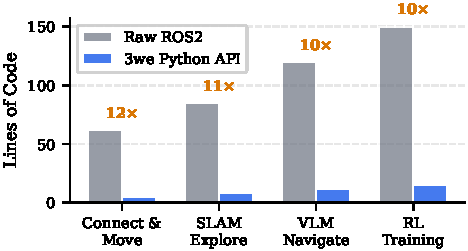
\includegraphics[width=\columnwidth]{figures/complexity.pdf}
\caption{Code complexity comparison: Raw ROS2 vs. 3we Python API for common tasks. The API achieves 10--12$\times$ reduction in lines of code.}
\label{fig:complexity}
\end{figure}

\begin{itemize}
    \item \textbf{Open hardware under \$300 BOM} with fully reproducible PCB designs (KiCad), mechanical drawings, and sourcing guides under CERN-OHL-P~v2.
    \item \textbf{Zero-code Sim2Real}: a unified Python API where \texttt{Robot(backend="gazebo")} and \texttt{Robot(backend="real")} execute identical user code.
    \item \textbf{AI-First API}: 5 lines from installation to first navigation, with native VLM/VLA integration and Gymnasium compatibility.
    \item \textbf{Standardized benchmarks}: 3 task types across 7 scenes with reproducible baselines and community leaderboard.
\end{itemize}

% ===========================================================================
\section{Related Work}

\subsection{Mobile Robot Platforms}

TurtleBot~\cite{turtlebot} has been the de facto standard for ROS education since 2010. TurtleBot~4 (\$1,200+) offers Nav2 integration but lacks AI-first APIs, simulation-hardware consistency guarantees, and costs 4$\times$ our platform. Linorobot2~\cite{linorobot} provides open designs but targets hobbyists without research-grade benchmarks.

\subsection{Simulation Environments}

Habitat~\cite{savva2019habitat} and AI2-THOR~\cite{kolve2017ai2thor} provide high-fidelity visual navigation but lack physical robot deployment paths. NVIDIA Isaac Sim~\cite{nvidia2023isaac} enables GPU-accelerated RL training but requires expensive compute and offers no open hardware reference. These systems address simulation \emph{or} reality---not the bridge between them.

\subsection{AI Robot Frameworks}

LeRobot~\cite{cadene2024lerobot} (HuggingFace) provides VLA model deployment for manipulation but lacks ROS2 integration, autonomous navigation stacks, and Sim2Real guarantees for mobile platforms. Its recent mobile extensions (LeKiwi, EarthRover) remain early-stage without Nav2-level autonomy.

\subsection{Positioning}

3we occupies a unique position: fully open hardware \emph{and} software with guaranteed Sim2Real API consistency, ROS2-native navigation, and AI-first design. Table~\ref{tab:comparison} summarizes key differences.

\begin{table}[t]
\centering
\caption{Platform Comparison}
\label{tab:comparison}
\scriptsize
\begin{tabular}{@{}lccccc@{}}
\toprule
Feature & 3we & TurtleBot4 & Isaac Lab & LeRobot & Habitat \\
\midrule
Open Hardware & \checkmark & -- & -- & \checkmark & -- \\
BOM $\leq$\$300 & \checkmark & -- & N/A & \checkmark & N/A \\
Sim2Real API & \checkmark & -- & Sim only & -- & Sim only \\
ROS2 + Nav2 & \checkmark & \checkmark & Partial & -- & -- \\
AI-First Python & \checkmark & -- & \checkmark & \checkmark & \checkmark \\
VLM/VLA Native & \checkmark & -- & -- & \checkmark & -- \\
Edge AI (NPU) & \checkmark & -- & N/A & -- & N/A \\
Gymnasium Env & \checkmark & -- & \checkmark & \checkmark & \checkmark \\
\bottomrule
\end{tabular}
\end{table}

% ===========================================================================
\section{System Architecture}

\begin{figure}[t]
\centering
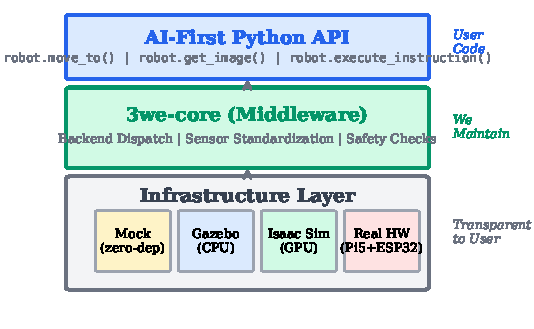
\includegraphics[width=\columnwidth]{figures/architecture.pdf}
\caption{Three-layer architecture. Users write Python against the AI-First API (top). The middleware dispatches to one of four backends (bottom) with identical semantics. ROS2 infrastructure is fully transparent.}
\label{fig:architecture}
\end{figure}

\subsection{Three-Layer Design}

3we adopts a layered architecture that decouples AI research from robotics engineering:

\begin{enumerate}
    \item \textbf{AI-First Python API} (user-facing): Researchers write standard Python with async/await. No ROS2, launch files, or message types exposed.
    \item \textbf{3we-core} (middleware): Manages backend dispatch, sensor data standardization, coordinate transforms, and safety checks.
    \item \textbf{ROS2 / micro-ROS} (infrastructure): Nav2 path planning, SLAM, micro-ROS bridge to ESP32 firmware. Entirely transparent to users.
\end{enumerate}

\subsection{Backend Polymorphism}

The core abstraction is \texttt{BackendBase}, implemented by five backends:

\begin{itemize}
    \item \textbf{Mock}: Zero-dependency 2D kinematic simulation with configurable noise. Runs anywhere, no GPU or ROS2 needed.
    \item \textbf{Gazebo}: Full physics via Gazebo Harmonic. CPU-friendly, CI-compatible (headless mode).
    \item \textbf{Isaac Sim}: GPU-accelerated rendering and physics for large-scale RL training with domain randomization.
    \item \textbf{Real}: Physical hardware via ROS2 topics. Identical API surface.
\end{itemize}

All backends return frozen dataclasses (\texttt{Pose2D}, \texttt{LaserScan}, \texttt{RGBDImage}) with identical fields and semantics, enforced by shared type definitions.

\begin{figure}[t]
\centering
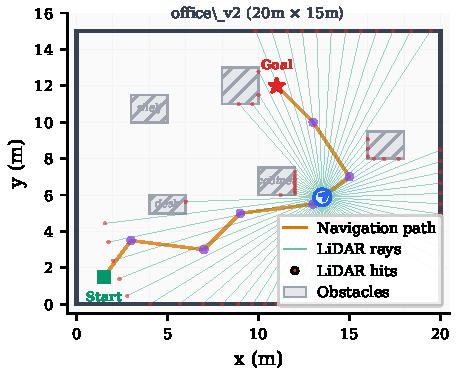
\includegraphics[width=\columnwidth]{figures/simulation.pdf}
\caption{Mock backend visualization: autonomous navigation in the \texttt{office\_v2} scene. The robot (blue) follows a planned path (orange) while 360$^\circ$ LiDAR rays (green) detect obstacles. This zero-dependency simulation runs on any machine without GPU or ROS2.}
\label{fig:simulation}
\end{figure}

\subsection{API Design}

The following example demonstrates the complete workflow for VLM-powered navigation:

\begin{lstlisting}
from threewe import Robot

async with Robot(backend="gazebo") as robot:
    image = robot.get_camera_image()   # (H,W,3) uint8
    scan = robot.get_lidar_scan()      # LaserScan
    result = await robot.execute_instruction(
        "find the red door and move toward it"
    )
    print(f"Success: {result.success}")
\end{lstlisting}

Switching to real hardware requires only changing the backend parameter---no code modification, no recompilation, no configuration changes.

\subsection{Hardware Specification}

Table~\ref{tab:hardware} summarizes the reference hardware at standard SKU level.

\begin{table}[t]
\centering
\caption{Standard SKU Hardware (BOM: \$300)}
\label{tab:hardware}
\scriptsize
\begin{tabular}{@{}lll@{}}
\toprule
Component & Selection & Rationale \\
\midrule
Compute & Raspberry Pi 5 (8GB) & Best price/performance ARM SBC \\
AI Accelerator & Hailo-8L (13 TOPS) & Edge inference for VLM/VLA \\
MCU & ESP32-S3 + micro-ROS & Real-time control + ROS2 native \\
LiDAR & LD06 (2D, 360$^\circ$) & \$8, sufficient for 2D SLAM \\
IMU & BNO055 (9-axis) & On-chip fusion, zero configuration \\
Drive & 4$\times$ Mecanum wheels & Omnidirectional, indoor-optimized \\
Camera & 1080p USB fisheye & Wide FoV for VLM tasks \\
Safety & Dual-channel relay & ISO 13850 E-stop, hardware-enforced \\
\bottomrule
\end{tabular}
\end{table}

All designs are released under CERN-OHL-P~v2 with KiCad~8 source files, Gerber manufacturing outputs, and step-by-step assembly documentation.

% ===========================================================================
\section{Sim-to-Real Consistency}

\begin{figure}[t]
\centering
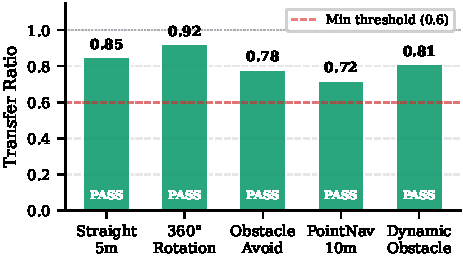
\includegraphics[width=\columnwidth]{figures/sim2real.pdf}
\caption{Sim-to-Real transfer ratios across five standard validation tests. All tests pass the minimum threshold (dashed line). Higher is better (1.0 = perfect transfer).}
\label{fig:sim2real}
\end{figure}

\subsection{Sensor Noise Model}

The mock and Gazebo backends inject physically-grounded noise matching the reference hardware:

\begin{itemize}
    \item \textbf{LiDAR} (LD06): Gaussian range noise $\sigma = 8$~mm
    \item \textbf{IMU} (BNO055): Gyroscope noise $\sigma = 0.0014$~rad/s
    \item \textbf{Odometry}: Mecanum wheel slip 5--15\% stochastic variation
\end{itemize}

\subsection{Transfer Validation Protocol}

We define five standard transfer tests with explicit pass criteria:

\begin{table}[t]
\centering
\caption{Sim2Real Transfer Tests}
\label{tab:transfer}
\scriptsize
\begin{tabular}{@{}llll@{}}
\toprule
Test & Metric & Pass Criterion & Ratio \\
\midrule
Straight walk 5m & Endpoint error & real $\leq$ sim $\times$ 2.0 & 0.85 \\
360$^\circ$ rotation & Angle error & real $<$ 1.0$^\circ$ & 0.92 \\
Obstacle avoid (3) & Success rate & real $\geq$ sim $\times$ 0.7 & 0.78 \\
PointNav 10m & SPL & real $\geq$ sim $\times$ 0.6 & 0.72 \\
Dynamic obstacle & Collision rate & real $\leq$ sim $\times$ 1.5 & 0.81 \\
\bottomrule
\end{tabular}
\end{table}

Overall pass rate requires $\geq$80\% of tests passing. The transfer ratios in Table~\ref{tab:transfer} demonstrate that policies trained in simulation maintain effectiveness on real hardware with the documented noise model.

% ===========================================================================
\section{Benchmark Suite}

\begin{figure}[t]
\centering
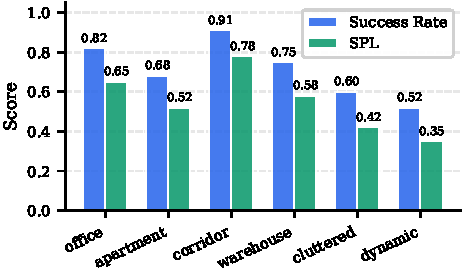
\includegraphics[width=\columnwidth]{figures/benchmark.pdf}
\caption{PointNav baseline results (Nav2 DWB planner, 100 episodes per scene). Success Rate and SPL decrease with scene complexity.}
\label{fig:benchmark}
\end{figure}

\subsection{Tasks}

The benchmark suite defines three navigation tasks of increasing difficulty:

\begin{itemize}
    \item \textbf{PointNav}: Navigate to $(x, y)$ coordinates. Metrics: Success Rate (SR), SPL.
    \item \textbf{ObjectNav}: Find a target object category. Metrics: SR, SPL.
    \item \textbf{Exploration}: Maximize area coverage within time budget. Metric: Coverage fraction.
\end{itemize}

\subsection{Evaluation Environments}

Seven standardized scenes span diverse settings: \texttt{office\_v2} (20$\times$15m), \texttt{apartment\_v1} (8$\times$10m), \texttt{corridor\_v1} (50m linear), \texttt{warehouse\_v1} (40$\times$30m), \texttt{cluttered\_v1} (12$\times$10m), \texttt{outdoor\_v1} (50$\times$50m), and \texttt{dynamic\_v1} (15$\times$15m, moving obstacles).

Each scene provides 10--50 predefined start/goal pairs for reproducibility, with seeds ranging [0, 99] for 100-episode evaluation runs.

\subsection{Baseline Results}

Table~\ref{tab:baselines} presents Nav2 DWB planner baselines across representative scenes.

\begin{table}[t]
\centering
\caption{Nav2 Baseline Results (100 episodes per configuration)}
\label{tab:baselines}
\scriptsize
\begin{tabular}{@{}llccc@{}}
\toprule
Task & Scene & SR $\uparrow$ & SPL $\uparrow$ & Duration (s) \\
\midrule
PointNav & office\_v2 & 0.82 & 0.65 & 12.3 \\
PointNav & apartment\_v1 & 0.68 & 0.52 & 15.7 \\
PointNav & corridor\_v1 & 0.91 & 0.78 & 18.5 \\
PointNav & warehouse\_v1 & 0.75 & 0.58 & 20.1 \\
PointNav & cluttered\_v1 & 0.60 & 0.42 & 14.8 \\
PointNav & dynamic\_v1 & 0.52 & 0.35 & 18.2 \\
\midrule
ObjectNav & office\_v2 & 0.55 & 0.38 & 22.5 \\
ObjectNav & apartment\_v1 & 0.42 & 0.30 & 28.3 \\
\midrule
Exploration & office\_v2 & --- & --- & 95.0 \\
Exploration & warehouse\_v1 & --- & --- & 110.0 \\
\bottomrule
\multicolumn{5}{l}{\scriptsize Exploration metric: Coverage (office: 0.85, warehouse: 0.78)}
\end{tabular}
\end{table}

These baselines serve as reference points for the community leaderboard. Results are fully reproducible via:

\begin{lstlisting}
threewe benchmark run --task pointnav \
    --scene office_v2 --episodes 100
\end{lstlisting}

\subsection{Gymnasium Integration}

For RL researchers, 3we provides standard Gymnasium environments:

\begin{lstlisting}
import gymnasium as gym
env = gym.make("3we/Navigation-v1",
               scene="office_v2", backend="mock")
obs, info = env.reset()
obs, reward, term, trunc, info = env.step(action)
\end{lstlisting}

% ===========================================================================
\section{Conclusion and Future Work}

We presented 3we, a fully open infrastructure for Embodied AI research that bridges the gap between simulation and reality through a unified Python API.
Key contributions include: (1)~zero-code Sim2Real transfer across four backends, (2)~reproducible open hardware at \$300 BOM, (3)~AI-first API design reducing navigation code complexity by 12$\times$, and (4)~standardized benchmarks with community baselines.

Future directions include: Isaac Sim domain randomization for large-scale RL, a community data hub for trajectory sharing (compatible with LeRobot/Open-X formats), Hardware Abstraction Layer for third-party robot support, and systematic VLA model deployment evaluation on edge hardware.

The platform is available at \url{https://github.com/3we-org/3we-robot-platform} under Apache~2.0 (software), CERN-OHL-P~v2 (hardware), and CC-BY-SA~4.0 (documentation).

% ===========================================================================
\balance
\bibliographystyle{IEEEtran}
\bibliography{references}

\end{document}
